%
% (C) Copyright 2000 Diomidis Spinellis.  All rights reserved.
%
% $Id$
%

\documentclass[10pt]{article}
\usepackage{mathptmx}
\usepackage{courier}
\usepackage[T1]{fontenc}
\usepackage{textcomp}

\usepackage{epsfig}
\usepackage{listings}

% listings language set
\lstdefinelanguage{PROJECTXML}
{morekeywords={project,id,scientific_coordinator,type,project_manager,shortname,projtitle,startdate,web_site,funding_agency,
funding_programme,project_code,enddate,partner,shortname,country,web_site,group},
sensitive=false
}

\lstdefinelanguage{PROJECTXSLT}
{morekeywords={xsl,template,match,mode,value,of,select,element,name,attribute,if,test},
sensitive=false
}

% See the dvips documentation
% Shrink figures larger than the text width to the text width
\def\epsfsize#1#2{\ifdim#1>\columnwidth\columnwidth\else#1\fi}
%\def\epsfsize#1#2{\textwidth}
\epsfverbosetrue

\title{Declarative Implementation of Semi-dynamic Web Sites}

\author{Diomidis Spinellis and Vassilios Karakoidas\\
Department Management Science and Technology \\
Athens University of Economics and Business \\
Greece\\
email: \{dds,bkarak\}@aueb.gr}

\date{}

\begin{document}

\maketitle

\begin{abstract}
\noindent
Traditionally, the realization of Web sites involves either
static content developed using web authoring tools like
Microsoft's Front Page and DreamWeaver, or dynamic
content delivered by a database driven front-end,
where the structured content is organized
in a relational schema and dynamically generated on the fly.
The limitations of statically-authored web pages are easy to discern and
for a number of applications, the use of a database
introduces a level of additional complexity that
makes the choice a part of the problem space rather than the solution space.
We introduce a different approach, which is suitable for managing 
middle-sized semi-dynamic web sites. The technological requirements of this
approach are well-known open source tools, such as CVS and XML.
\end{abstract}

\subsection*{Keywords}
Web applications, XML, make, Bibtex, XSLT, DTD

\section{Introduction}
\label{sec:intro}
Traditionally, the realization of Web sites involves either
static content developed using web authoring tools like
Microsoft's Front Page and DreamWeaver, or dynamic
content delivered by a database driven front-end,
where the structured content is organized
in a relational schema and dynamically generated on the fly.
When our group faced the successive failure of both the above approaches,
we decided to adopt the task of exploring ideas for a radically different
implementation style, based on the declarative specification
of all the site's elements.
We believe that our approach and many of the lessons we learned
can be applied numerous similar situations,
leading to a lightweight, structured, consistent, and maintainable
web site building method.

The limitations of statically-authored web pages are easy to discern.
The content is entered in an unorganized manner, and, as a result,
can be inconsistent in both structure and presentation.
While the use of cascading style sheets can help one obtain a
consistent look, their use still requires discipline.
The authored pages are however still unstructured and the resulting
site can be difficult to modify and reorganize.
Furthermore, the static authoring model often imposes a centralized
management and maintenance style;
all additions and changes have to go through a single person,
creating a bottleneck, often leading to outdated content.

Adopting a database driven approach is supposed to
solve the problems we described.
Separating the content's data from its (dynamically generated)
presentation leads to a consistent
yet flexible presentation style.
In addition, the database's relational model will impose
its structure on the data being stored.
Finally, the use of a database, allows concurrent updates by
different users.

However, for a number of applications, the use of a database
introduces a level of additional complexity that
makes the choice a part of
the problem space rather than the solution space.
A database-driven web site requires the implementation of a
front-side interface to transform the database content into
{\sc html} code, and a back-end interface to allow stakeholders
enter, review, and update data.
The back-end client interface typically requires setting up
and maintaining appropriate access permissions.
These may need to be integrated into an organization wide single
login facility, or operated under a specific security policy.
In the second case procedures for setting up passwords,
resetting them, and revoking them need to be established
 for a number of applications, the use of a database
introduces a level of additional complexity that
makes the choice a part of
the problem space rather than the solution space.and followed.
A properly running database also requires a skilled database
administrator to install it, maintain it, organize backups,
and perform modifications to the database schema.
In addition, because content is generated by a front-end
program accessing the database, both the front-end and the database
must be extremely robust, running on a $24 \times 7$ schedule.
The front-end, being an executable program working on
untrusted data (the web page requests) can become the target of
malicious attacks,
and must therefore be inspected to ensure its robustness.
To minimize the risk of an attack against the database
(that would jeopardize the organization's data)
the database server has to be installed on a machine separate
from the web server, behind a (properly configured) firewall.
Finally, the extraction of content from a database often
induces the web site's designers and stakeholders adopt a
query-style interface.
Such an interface is typically less usable than browsable web pages,
and the served content is often ignored by search engines,
leading to reduced visibility
of the (meticulously structured) content.
All in all, a database-driven approach appears to be suitable
only for those with ample resources to justify the full
development and appropriate maintenance of a sophisticated infrastructure.

At the time we volunteered to take up the project of managing our
research center's web site, the site had already undergone through
the two approaches we described.
An ad-hoc authoring tool--based approach was abandoned,
because it led to an inconsistent look and stale content,
while the maintenance of a subsequent database-oriented
design approach was proving intractable for the resources
our group could afford to commit.
Our goal for taking up the project, was to experiment with a
different approach,
proving its suitability for managing middle-sized semi-dynamic
web sites.

\section{Requirements}
\label{sec:req}
\begin{figure}
\begin{center}
\leavevmode
\epsfbox{Diag.eps}
\end{center}
\caption{
\label{fig:diag}
Overview of data element relationships.}
\end{figure}
The functional requirements for our center's site were
simple, but not trivial, and had already been satisfied
twice in a slightly simpler form.
The site's pages should represent the content and the relationships
we illustrate in Figure \ref{fig:diag}.
The center consists of multiple research groups.
Members of our center and our research projects are
associated with the center as a whole, and, typically, also
with one or more research groups.
Publications, such as journal articles and books,
are also associated with the center, individual members (the authors),
projects that funded the corresponding work,
and groups that performed the work.
Note that members, publications, and projects associated
with one or more groups are aggregated are typically associated
again with the research center as a whole.
For the sake of simplicity,
we have omitted from our description and the diagram
a number of additional relationships,
such as the member directing a group or managing a project.
As an example of the type of content we were looking for,
the research center and
each member, group, or project should have a web page with a list
of the corresponding publications;
the research center and each group should have pages listing
their projects and members.

As we hinted in the previous paragraph, the problem with
the previous implementations was not the creation of the site
satisfying the functional specifications,
but the lack of a number of important non-functional properties.
Before embarking on our third attempt,
we articulated for the first time those non-functional requirements
we thought important, to ensure that our third attempt would produce
a result with a longer life.
The following is a list of the non-functional properties
we deemed important enough to guide our design.

\begin{description}
\item[Openness] The tools used in the realization
should be available as open soueditorrce, or sourced by multiple vendors.
We wanted to avoid becoming tied with a particular proprietary
tool.
We reasoned that openness would mitigate two risks:
finding a maintainer trained to use a particular proprietary tool,
and obtaining resources for upgrading and maintaining the tool.

\item[Observability]
We should try to minimize,
to the greatest extend possible, the semantic distance between
the specification of an element and its implementation \cite{SG97}.
The site's look and content should be maintainable
using standard tools and techniques.
If possible, the site's maintainer should not be required to
learn a scripting language like {\sc php}, or Perl, or
a framework like Java2EE or {\sc .net}.
An approach based on declarative specifications and
domain-specific languages would allow end-users, or members
close to end-users be involved in maintaining the site,
without risking the bottleneck of going through
multiple intermediaries.

\item[Robustness] The web site should not depend on
any programs other than the web server for serving
its content.
Users updating the data, should be able to author, validate and 
review, generating localy the HTML pages, 
their changes without requiring network connectivity.
This would allow them to work productively over dial-up connections
or while on the road. In addition, all the editing can be done with 
a simple text editor and the each end-user can work both in win32 and unix oriented systems.
Minimizing the dependencies on additional servers (such as a
database or an application server) and on the network
should result in a more robust and easier to maintain system.   

\item[Parsimony] The implementation effort for
implementing the system should be minimal.
This would minimize errors and maintenance costs.
We reasoned we could satisfy this requirement by
using existing tools, if their choice satisfied the
other non-functional requirements.

\end{description} 

\section{Design Process}
\label{sec:design}
\begin{figure}
\begin{center}
\leavevmode
\def\epsfsize#1#2{\epsfxsize}
\epsfysize.8\vsize
\epsfbox{rankyear.eps}
\end{center}
\caption{
\label{fig:rankyear}
Yearly changes in web site rankings.}
\end{figure}

\subsection{Key Technologies}

In order to meet the requirements we set in section 2, we decided to adopt open and popular
technologies as key elements of our system. For data representation we used XML and bibtex.\\
XML ...\\
Bibtex ...\\
To deal with the problem of versioning and multi-persion development we used CVS. CVS ...\\
The simple tasks of our systems were automated using a make file. Make is ...\\

\subsection{Design Concepts}

The guiding paradigm we adopted for designing the process
for implementing the web site was that the task was essentially
a continuous multi-person development activity.
Live web sites continuously evolve;
adopting the content authoring paradigm implied
by the first approach we tried was a mistake.
Empirical evidence supports this observation.
Figure \ref{fig:rankyear} illustrates the changes
in rankings given to 21 Greek government department
web sites between the years 2002 and 2003.
The X shape in the rank changes between the one year and the next
is, we believe, the result of statically authored web pages
degrading to a point of irrelevance, and then being overhauled
from scratch.
A database-driven approach also hinders evolution.
Changes to the content's presentation require the modification
and installation of the front end page generator;
not a typical lightweight operation.
Changes to the data schema are even more intrusive
requiring a synchronized modification of the data,
the front end, and the back end.

\begin{figure}
\lstset{language=XML,basicstyle=\ttfamily}
{\begin{lstlisting}
<!ELEMENT project (
  shortname, projtitle, startdate?, 
  enddate, web_site?, funding_agency?, 
  funding_programme?, project_code?, partner*,
  logo?, description)>
<!ATTLIST project
  id ID #REQUIRED group IDREFS #REQUIRED
  scientific_coordinator IDREF #IMPLIED
  project_manager IDREF #IMPLIED
  type (consulting | rtd | training | dissemination) #REQUIRED >
\end{lstlisting}}
\caption{The projects DTD file}
\label{fig:project-dtd}
\end{figure}

\begin{figure}
\lstset{language=PROJECTXML,basicstyle=\ttfamily}
{\begin{lstlisting}
<project id="p_mexpress"
  group="g_eltrun g_sense g_wrc" scientific_coordinator="m_dds"
  type="rtd" project_manager="m_pateli">
  <shortname>mExpress</shortname>
  <projtitle>mobile in-EXhibition PRovision 
  of Electronic Support Services</projtitle>
  <startdate>20020305</startdate>
  <enddate>20040401</enddate>
  <web_site>http://mexpress.intranet.gr/</web_site>
  <funding_agency>European Commission</funding_agency>
  <funding_programme>IST</funding_programme>
  <project_code>IST-2001-33432</project_code>
  <partner>
    <shortname>Ericsson</shortname>
    <country>DK</country>
    <web_site>http://www.ericsson.com/</web_site>
  </partner>
</project>
\end{lstlisting}}
\caption{A typical project XML file}
\label{fig:project-xml}
\end{figure}

\begin{figure}
\lstset{language=PROJECTXSLT,basicstyle=\ttfamily}
{\begin{lstlisting}
<xsl:template match="project" mode="full">
  <h1> 
  	<xsl:value-of select="shortname" /> -
	<xsl:value-of select="projtitle" /> 
  </h1>
  <xsl:element name="img">
  	<xsl:attribute name="src">
		<xsl:value-of select="logo" />
	</xsl:attribute>
  </xsl:element>
  <br /> <br />
  <xsl:if test="count(project_code) != 0">
    	Project Code: 
	<xsl:value-of select="project_code" />
	<xsl:if test="@international = 'yes'">
		(International)
	</xsl:if> 
	<br/>
</xsl:if>
\end{lstlisting}}
\caption{The XSLT transformation file for projects}
\label{fig:project-xslt}
\end{figure}

\begin{figure}
\lstset{language=HTML,basicstyle=\ttfamily}
{\begin{lstlisting}
<html>
<head>
	<meta http-equiv="Content-Type" 
	 content="text/html; charset=UTF-8">
	<!--Generated by $Id: declweb.tex,v 1.2 
	 2004/02/19 23:34:28 dds Exp $-->
	<title>ELTRUN  - Project Details</title>
</head>
<body>
  <h1>
  mExpress - mobile in-EXhibition 
  PRovision of Electronic Support Services
  </h1>
  <img src="../images/p_mexpress.gif" />
  <br /><br />
  Project Code: IST-2001-33432 (International) <br />
  Funding programme: IST<br />
  Funding Agency: European Commission<br />
  Project type: RTD<br/>editor<br />
  Web site:
  <a href="http://mexpress.intranet.gr/">
  http://mexpress.intranet.gr/
  </a><br /><br />
  Starting date: 5 March 2002<br/>
  Ending date: 1 April 2004<br />
  Scientific coordinator:
  <a href="../members/m_dds.html">
  Dr. Diomidis Spinellis
  </a><br />
  Project Manager:
  <a href="../members/m_pateli.html">
  Mrs. Ada Pateli
  </a><br>
</body>
</html>
\end{lstlisting}}
\caption{A generated HTML project file}
\label{fig:project-html}
\end{figure}

Continuous multi-person development projects are quite
common in software development.
Numerous developers contribute and coordinate their work
through a version control system, like {\sc cvs} that
maintains a master repository of the source code.
Concepts like the daily build \cite{CS95b} or the
{\em current} and {\em stable} branches as practiced by
numerous open source projects allow the maintenance
of a known-good product.
What we needed for our approach were appropriate
declarative language-based formalisms for expressing our data,
its transformation into {\sc html} pages, and the
generation process.yWe were clear that we wouldn't support he content in a {\em Makefile} \cite{OTT91}.
You can see representative samples of a project's
{\sc dtd} schema description in figure \ref{fig:project-dtd}.
{\sc Xml} data in figure \ref{fig:project-xml}.
{\sc Xslt} transformationn in figure \ref{fig:project-xslt},
and {\sc html} result in figure \ref{fig:project-html}.

\subsection{Processes}

\begin{figure}
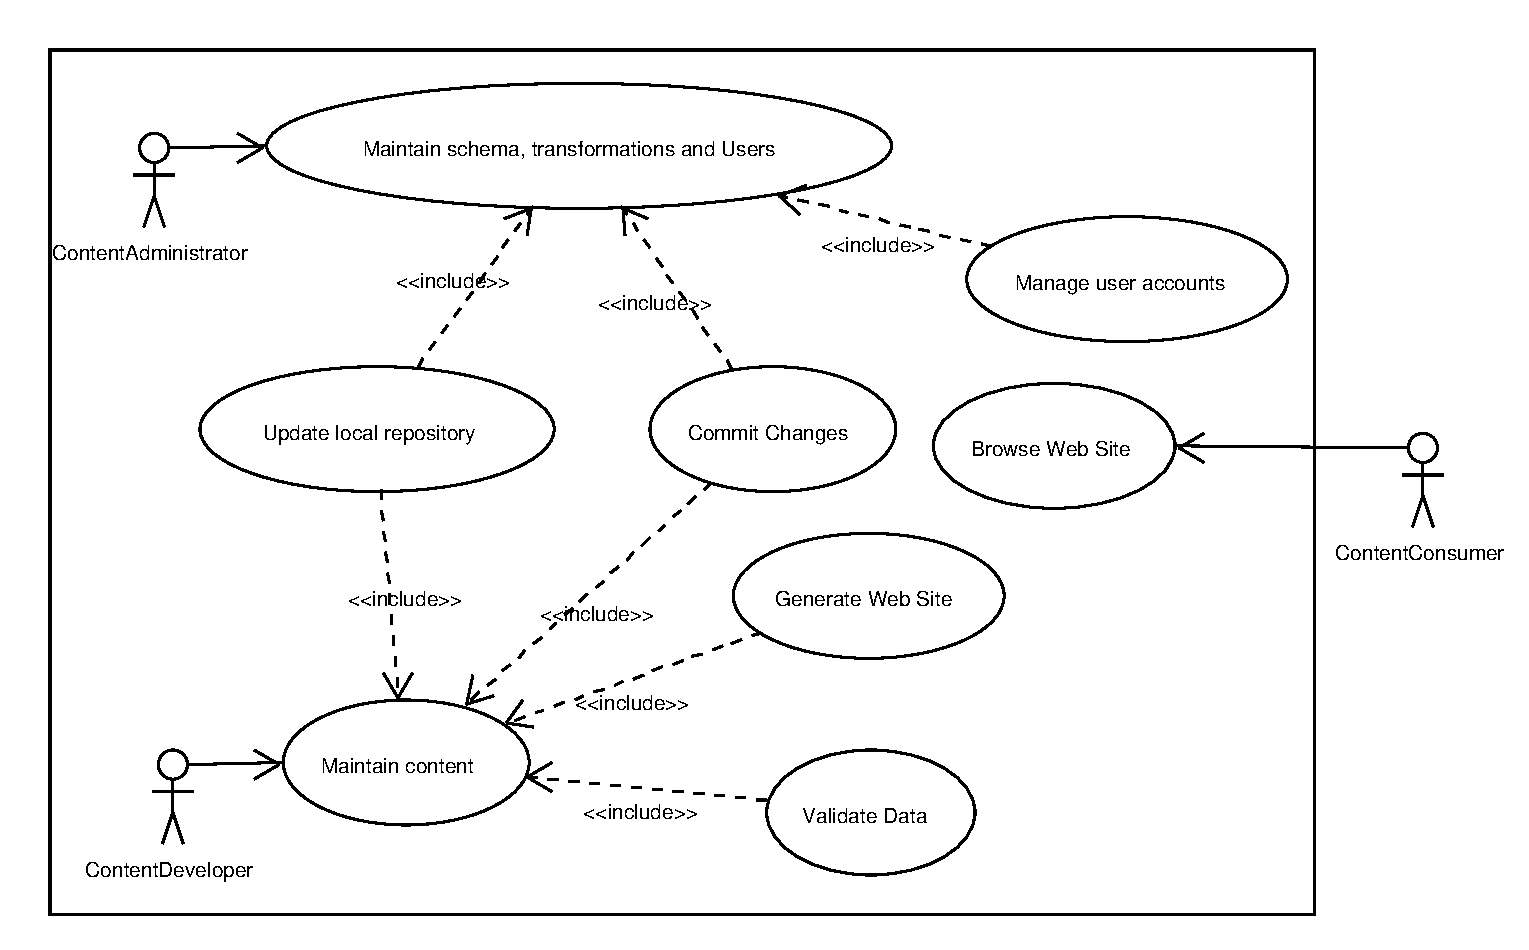
\includegraphics[scale=0.5]{use-case-diagram}
\caption{UML Use Case Diagram of the System}
\label{fig:use-case-diagram}
\end{figure}

In Figure \ref{fig:use-case-diagram} is depicted a UML use case diagram of our system. 
We have three actors which are interacting with the system:

\begin{description}
\item[ContentDeveloper] A content developer is responsible for uploading data in the system. In our case is typically a person for each research group. He can upload XML data files and import new bibliography entries.

\item[ContentAdministrator] The content administrator is responsible for the maintaince and the evolution of the framework. He corrects problems with the XML Data, develops new features or corrects existing ones in the XSLT scripts and the DTD schemas.

\item[ContentConsumer] The content consumers are outside our system and they have access only int the generated web site.
\end{description}

The use cases that comprise our system are:

\begin{figure}
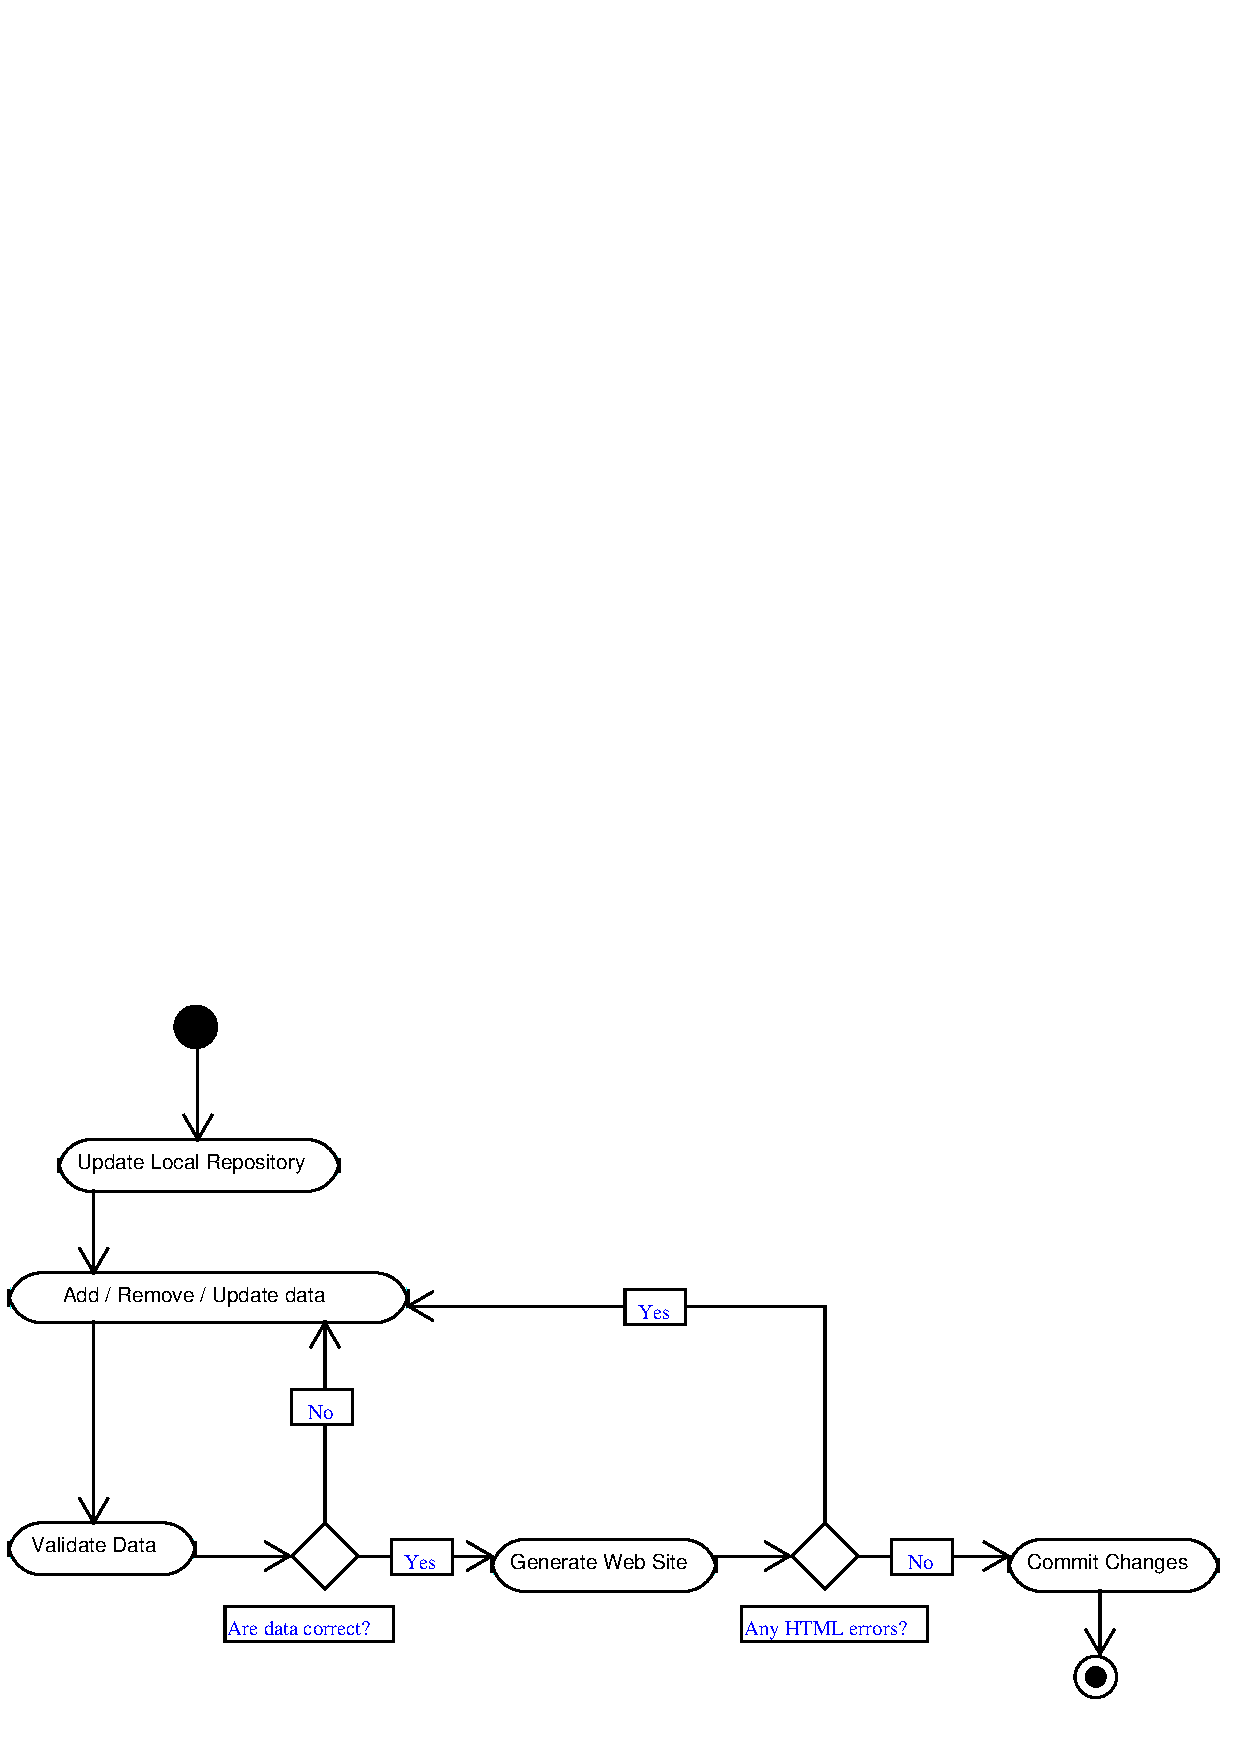
\includegraphics[scale=0.5]{maintain-content-activity}
\caption{UML activity diagram for Maintain Content}
\label{fig:maintain-content-diagram}
\end{figure}

\begin{description}
\item[Maintain Schemas, Transformations and Users]

\item[Update Local Repository]

\item[Commit Changes]

\item[Maintain Content] This use case is described with the acrivity diagram in Figure \ref{fig:maintain-content-diagram}.

\item[Generate Web Site]

\item[Validate Data]

\item[Manage User Accounts]

\item[Browse Web Site]

\end{description}

\section{Implementation}
Once the design was finalized,
implementation proved to be an almost ``hollow'' activity,
since it did not involve almost anything of what
is typically described as coding.

The first step involved selecting and setting up the
appropriate tools.
We adopted the concurrent versions system
({\sc cvs}) \cite{BF01} to coordinate the distribution
and update of all the system's elements.
Authentication for managing content was handled by the
Unix group membership mechanism of the host where the
{\sc cvs} repository was stored.
We also used
BibTeX and {\em bib2html} for transforming the publications
into {\sc html} and
{\em xmlstarlet} for validating and transforming
all other {\sc xml}-based data.
Finally, {\sc gnu} {\em make} and a couple of shell script
constructs were used for handling the project's {\em Makefile}.
The complete setup including all tools proved to be portable
between Unix and Microsoft Windows, with team members working
on machines running different versions of Windows, {\sc gnu}/Linux,
and Free{\sc bsd}.

The next step was a series of iterations where we
modeled the data's schema on representative {\sc xml}
files and concurrently wrote the validation {\sc dtd}s
and the transformation {\sc xslt}s.
The version control system was already proving its value
at this point
for coordinating the work between the two paper's authors.
Because many page elements, like a project's description,
could contain content more elaborate than plain text,
we used W3C's modular {\sc xhtml} specification for
importing existing {\sc xhtml} elements editorin our {\sc dtd}s.
This helped us keep our schema description simple,
but the corresponding schema expressive.

The automated validation and generation of content was
expressed as {\em Makefile} rules.
The individual files {\sc xml} files are merged in a
single {\sc xml} file for cross validating identifier
reference attributes ({\sc idref}).
The same file is used to extract the identifiers of
all projects, members, and groups into {\em Makefile}
variables.
A simple loop then generates the {\sc html} files
corresponding to each of the above elements.

The {\sc html} content is by default generated on the
local machine, where its maintainer can verify it.
After the new content is validated and verified,
the maintainer can commit the change to tWe were clear 
that we wouldn't support he master {\sc cvs} repository.
A separate {\em Makefile} rule can then be used,
to execute an update command on the
host serving the content to the web.
The command retrieves the updates from the {\sc cvs}
repository and regenerates the pages on the web-server's
file area.
As all elements of our system are under version control,
all pages are automatically tagged with identifiers
denoting their source, helping the traceability of changes.
All exchanges between the developers' machines and the
{\sc cvs} and web host are performed using the secure session
shell ({\sc ssh}) protocol guaranteeing the data's integrity
and confidentiality.

\begin{figure}
\includegraphics[scale=0.7]{distro.eps}
\caption{Directory structure of local repository}
\label{fig:eltrun-web-distro}
\end{figure}

Our framework has a distribution that works in both win32 and 
Unix Enviroments (Linux and FreeBSD). The directory structure of a typical local repository depicted in
figure \ref{fig:eltrun-web-distro}.
Most of our users are working in win32 enviroments and as 
a result we decided to upload a win32 version of the needed tools 
in the main repository under the directory "bin". The installation procedure is very simple,
and the bootstrap tools that requires are only cvs for 
the initial check out and a ssh client. The needed keys 
for the secure shell session are provided once in each user. 
A full version of the system now demands 8 megabytes of space 
in local machine, plus some extra for the local content store and generation.

\section{System Adoption}
\label{sec:adopt}
After we had finished the design we were somewhat concerned
by how the system would be received by those who would be
maintaining the pages.
Our research center is multidisciplinary: under its roof
are both hard core software engineers using the same tools
we adopted in their everyday work, and researchers whose
background is management science, marketing, or finance
who are comfortable with {\sc gui} interfaces.

Our fears were justified.
The first presentation of the system to its users ended
almost in a revolt.
Non-technical users expressed their inability to comprehend
what an {\sc xml} document was, while technical members
helpfully argued for providing a {\sc gui} front end.
By targeting the users with the least technical experience,
promoting our system's ``vogue'' attributes,
such as the use of open source software tools,
and convincing them to try to enter a few elements into
the system, we were able to overcome the initial reservations
and start the data migration process.

The next round of problems surfaced when users began entering
malformed or invalid data into the system.
This resulted in all users acquiring the copies of the malformed
{\sc xml} files, and strange error messages given to unsuspecting
users.
As is the custom in a number of development efforts, we had
expected the users to verify the changes they made before
committing them into the master repository.
Non-technical users were however not aware of this etiquette
and were committing their changes with the hope they were correct.
We used the shared list we had established to explain the
importance of following the correct procedures when committing changes.
After a few days we got the impression that non-technical users
were becoming confident in their work, even proud of sharing
sophisticated tools and processes with software engineers.

Two weeks after the initial system presentation all users where able to upload 
and maintain their data. The inexperienced users learned to edit XML files,
importing bibtex entries into the system and commiting to the common CVS repository. 
They just followed steps in procedure that they see as a black box. 
Our technical persons experienced more problems than the inexperienced ones 
and that was came as a suprise for us. Some of them were already familiar 
with the key technologies and they tried to change the tools proposed with others more user-friendly. 
These initiatives resulted in corruption of the local repositories, malformed XML data and wrong bibliography entries.
After a few false attempts they decided to follow the proposed framework.

\section{Lessons Learned}
\label{sec:concl}
We believe our design satisfies the non-functional specifications
we listed in Section \ref{sec:req},
and that our approach stands a higher chance to succeed where the
two other approaches failed.
The initial user reaction was not favorable, but this can
be explained by the significantly higher requirements we
placed on our users.
Instead of giving instructions by email to an unfortunate
web site maintainer, they now had to become active members
of an evolving web site maintenance effort.
Not all members of our research center proved ready to take
this responsibility.
Many groups delegated the maintenance to a single person.
Still, however, we succeeded in distributing the previously
entirely centralized maintenance effort across our groups.
Summarizing, we believe that adopting a software development
metaphor and tools for developing and maintaining semi-dynamic
web content is a practical worthwhile approach.

\bibliographystyle{unsrt}
\bibliography{declweb}

\end{document}
